\section{Модификация проекта «Выпуклая оболочка»}
\subsection*{Точная постановка задачи}
Вычисляется количество вершин выпуклой оболочки, лежащих в 1-окрестности заданного заполненного треугольника.
После запуска программа предлагает пользователю ввести последовательно координаты вершин выпуклой оболочки. Введённая точка индуктивно добавляется в
выпуклую оболочку. Нам же необходимо вместе со значениями периметра и площади
выпуклой оболочки выводить количество точек, попадающие в заданный заполненный треугольник или в его 1-окрестность. Для этого необходимо до начала ввода координат вершин выпуклой оболочки задать треугольник, потребовав на ввод 6 координат треугольника. 

  Это задание не требует серьёзной модификации исходного кода, все функции
будут вписываться в файлы проекта $\texttt{convex.rb}$ и $\texttt{r2point.rb}$.

\subsection*{Решение}
Эталонный проект до модификации индуктивно строит выпуклую оболочку по
точкам. При добавлении новой точки программа индуктивно перевычисляет периметр и
площадь оболочки. Наша цель "--- модифицировать эталонный проект таким 
образом, чтобы вычислялось количество вершин выпуклой оболочки, лежащих в 1-окрестности заданного заполненного треугольника.

  Для решения данной задачи необходимо проверять, принадлежат ли вершины выпуклой оболочки
заданному треугольнику или 1-окрестности заданного треугольника. В языке Ruby имеется библиотека $\texttt{Math}$, которая содержит
методы вычисления простейших тригонометрических функций, в частности, в данном проекте используется $\texttt{Math.sqrt}$.

  После добавления вершины выпуклой оболочки возникает три случая, которые необходимо рассмотреть: 
\begin{enumerate}
\item вершина находится в заполненном треугольнике;
\item вершина находится в единичной окрестности треугольника;
\item вершина находится вне треугольника и единичной окрестности.
\end{enumerate}
\subsubsection*{Вершина находится в заполненном треугольнике}
  Для того, чтобы проверить, лежит ли точка в треугольнике мы будем использовать псевдоскалярное произведение~\cite{psevdoscalyar}. 2 вершины треугольника образуют отрезок, который можно воспринять как луч. Этот луч делит всю плоскость на 2 полуплоскости. Берутся 2 вершины треугольника и обозреваемая точка, затем относительно них выполняется псевдоскалярное произведение.
\begin{center}
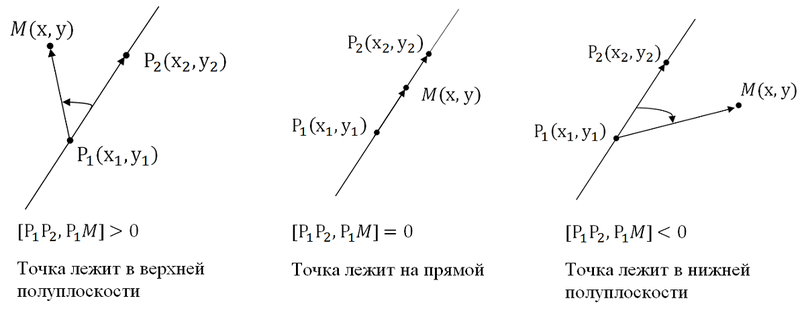
\includegraphics[width=0.9\hsize]{images/psevd}
\end{center}
 Знак числа, которое получается при вычислении говорит нам, в какой из полуплоскостей относительно стороны треугольника лежит точка. Если все знаки чисел, полученных во время вычисления псевдоскалярных произведений относительно всех сторон треугольника, совпадают, значит точка лежит внутри треугольника, иначе, точка находится вне треугольника.
\subsubsection*{Вершина находится в единичной окрестности треугольника}
   Для определения принадлежности точки единичной окрестности мы будем считать расстояние от точки до сторон треугольника. Если хотя бы одно из этих расстояний находится в промежутке (0,1), то точка находится в единичной окрестности заданного треугольника. Для определения расстояния от точки надо сначала определить, лежит ли точка левее или правее отрезка. Вычисляется скалярное произведение от искомой точки до каждого из карев отрезка.
Если одно из этих скалярных произведений меньше или равно нулю, то возвращается расстояние от точки до края отрезка, скалярное произведение с которым было меньше либо равно нулю, причем считается расстояние как гипотенуза прямоугольного треугольника. Если же скалярные произведения больше нуля, то расстояние считается по формуле, которая указана ниже~\cite{rasst}.

$$d\bigr(P,L)=\frac{(y_{0}-y_{1})x+(x_{1}-x_{0})y+(x_{0}y_{1}-x_{1}y_{0})}{\sqrt{(x_{1}-x_{0})^2+(y_{1}-y_{0})^2}}.$$

 
\subsection*{Модификация кода}
Для начала модифицируем файл $\texttt{convex/r2point.rb}$ добавив в класс $\texttt{R2Point}$ методы,
которые выполняют следующие действия:

\medskip
\begin{itemize}
\item нахождение расстояния от точки до отрезка;
\item проверка принадлежности точки треугольнику;
\item проверка принадлежности точки окрестности и треугольнику.
\end{itemize}

\begin{small}
\begin{verbatim}
def dist_segm(a,b)
  p1=(@x-a.x)*(b.x-a.x)+(@y-a.y)*(b.y-a.y) 
  p2=(a.x-b.x)*(@x-b.x)+(a.y-b.y)*(@y-b.y)
  return Math.sqrt((@x-a.x)**2+(@y-a.y)**2) if p1<=0 
  return Math.sqrt((@x-b.x)**2+(@y-b.y)**2) if p2<=0 
  a=(a.y-b.y)*@x+(b.x-a.x)*@y+(a.x*b.y-b.x*a.y
  b=Math.sqrt((b.x-a.x)**2+(b.y-a.y)**2)
  return (a/b).abs 
end
\end{verbatim}
\end{small}   

Метод $\texttt{dist\_segm(a,b)}$ возвращает расстояние от точки, к которой применяется этот метод до отрезка, концами которого являются точки $\mathit a$ и $\mathit b$.

\begin{small}
\begin{verbatim}
def inside_triangle?(a,b,c)
  l=(a.x-@x)*(b.y-a.y)-(b.x-a.x)*(a.y-@y)
  m=(b.x-@x)*(c.y-b.y)-(c.x-b.x)*(b.y-@y)
  n=(c.x-@x)*(a.y-c.y)-(a.x-c.x)*(c.y-@y)
  (l>0 && m>0 && n>0) || (l<0 && m<0 && n<0)
end
\end{verbatim}
\end{small} 

Метод $\texttt{inside\_triangle?(a,b,c)}$ использует псевдоскалярное произведение для определения, находится ли точка внутри треугольника. Если точка, к которой применяется этот метод находится внутри треугольника, то метод возвращает true, иначе возвращается false

\begin{small}
\begin{verbatim}
def is_inside?(a,b,c)
  return true if self.inside_triangle?(a,b,c) #если в треугольнике
  return true if (self.dist_segm(a,b)<=1 && self.dist_segm(a,b)>=0) ||
  (self.dist_segm(b,c)<=1 && self.dist_segm(b,c)>=0) ||
  (self.dist_segm(c,a)<=1 && self.dist_segm(c,a)>=0) || 
  (self.dist_segm(a,c)<=1 && self.dist_segm(a,c)>=0)
  return false
end
\end{verbatim}
\end{small} 

Метод $\texttt{is\_inside?(a,b,c)}$ выполняет финальную проверку на принадлежность точки треугольнику или окрестности треугольника. Первоначально, он проверяет, лежит ли точка внутри треугольника, вызывая метод $\texttt{inside\_triangle?(a,b,c)}$. Если этот метод вернул true, то и метод $\texttt{is\_inside?(a,b,c)}$ возвращает true, говоря о том, что точка удовлетворяет условию. Если же был получен false, то идет проверка окрестности. Проверяется расстояние от точки до каждой из сторон при помощи метода $\texttt{dist\_segm(a,b)}$. Если хотя бы до одной стороны расстояние больше нуля и меньше единицы, то возвращается true, опять же говоря о том, что точка удовлетворяет условию. Во всех остальных ситуациях (если точка не лежит ни в треугольнике, ни в окрестности) возвращается false, что означает, что точка не удовлетворяет условию и увеличивать количество точек, удовлетворяющих условию, не стоит.

Теперь модифицируем файл $\texttt{convex/convex.rb}$. Добавим в класс $\texttt{Figure}$  инициализацию объекта, метод создания треугольника, метод проверки
на принадлежность треугольнику и метод получения количество вершин выпуклой оболочки, которые удовлетворяют нашему условию.

\begin{small}
\begin{verbatim}
def initialize; @ins=0 end
\end{verbatim}
\end{small}

Теперь при инициализации абстрактной фигуры создается переменная экземпляра класса  $\texttt{Figure @ins}$ . Так как в нашем проекте создается только одна выпуклая
оболочка, мы можем использовать именно этот тип переменной.

\begin{small}
\begin{verbatim}
def set_triangle(a,b,c)
  @@a, @@b, @@c = a,b,c
end
\end{verbatim}
\end{small}

Задание треугольника производится тремя точками, которые будут храниться в переменных класса  $\texttt{Figure @@a, @@b, @@c}$ соответственно. Так как при добавлении вершин выпуклой оболочки может произойти создание объекта другого класса, нам придется использовать именно переменные класса, ибо все объекты классов 
$\texttt{Void, Point, Segment, Polygon}$ наследуются от класса $\texttt{Figure}$, а следовательно, наследуют и точки нашего треугольника.

\begin{small}
\begin{verbatim}
def intr?(p) ; (p.is_inside?(@@a,@@b,@@c)) ? 1 : 0 ;end
\end{verbatim}
\end{small}

Метод $\texttt{intr?(p)}$ проверяет принадлежность точки, получаемой в качестве аргумента, заданному ранее треугольнику используя метод $\texttt{is\_inside?(a,b,c)}$, который возвращает true, в случае, если точка лежит 
либо в заданном треугольнике, либо в его единичной окрестности и false во всех остальных случаях. Метод  $\texttt{intr?(p)}$, в случае, если точка попадает в заданный треугольник или его окрестность, возвращает число 1, во всех остальных
случаях он возвращает 0.


\begin{small}
\begin{verbatim}
def inside_points; @ins; end 
\end{verbatim}
\end{small}

Метод $\texttt{inside\_points}$ возвращает переменную экземпляра  $\texttt{@ins}$, которая хранит количесто вершин, лежащих в заданном треугольнике или его единичной окрестности.

Теперь рассмотрим класс  $\texttt{Void}$. Так как объект именно этого класса создается при начале работы программы, то 
задавать треугольник лучше всего именно в нем. Для этого добавим инициализацию объекта класса $\texttt{Void}$.

\begin{small}
\begin{verbatim}
def initialize(a=R2Point.new, b=R2Point.new, c=R2Point.new)
  set_triangle(a,b,c)
end
\end{verbatim}
\end{small}

Если при создании объекта класса $\texttt{R2Point}$ не указать аргументы, то координаты точки будут запрашиваться
через ручной ввод, мы этим воспользуемся. Зададим 3 точки $\texttt{a, b, c}$ и передадим их в метод $\texttt{set\_triangle(a,b,c)}$, чтобы задать эти точки как переменные класса $\texttt{Figure}$, которые в будущем будут
доступны из всех классов.

После задания треугольника можно начать работать с точками выпуклой оболочки. В классе $\texttt{Point}$ изменим 
инициализацию, добавив строчку, которая будет проверять, лежит ли она в заданном ранее треугольнике или его единичной окрестности.

\begin{small}
\begin{verbatim}
class Point < Figure
  def initialize(p) 
    @p = p
    @ins=intr?(@p) 
  end
  ...
end
\end{verbatim}
\end{small}

Если точка удовлетворяет условию, то переменная $\texttt{@ins}$ будет равна 1, в противном случае, она будет равна 0, так как метод $\texttt{intr?(p)}$ возвращает 1, если точка удовлетворяет условию и 0, если не удовлетворяет.

По тому же принципу изменим инициализацию класса $\texttt{Segment}$ и класса $\texttt{Polygon}$

\begin{small}
\begin{verbatim}
class Segment < Figure
  def initialize(p, q) 
    @p, @q = p, q
    @ins=intr?(@p)+intr?(@q)
  end
  ...
end

class Polygon < Figure
  attr_reader :points, :perimeter, :area 
  ...
  @area      = R2Point.area(a, b, c).abs
  @ins=intr?(a)+intr?(b)+intr?(c)
  end
\end{verbatim}
\end{small}




Также нам нужно будет проверить пересекаются ли прямые, на которых лежит ребро выпуклой оболочки и 
заданный отрезок. Для этого добавим в файл $\texttt{convex/convex.rb}$ метод $\texttt{cross?}$ в класс 
$\texttt{Segment}$, который будет проверять данное условие.

\begin{small}
\begin{verbatim}
def cross?(point1,point2)
 if (point1.x==point2.x && self.p.x==self.q.x)
  return false
 else
  an=(point2.y-point1.y)/(point2.x-point1.x)
  bn=(self.q.y-self.p.y)/(self.q.x-self.p.x)
  if an == bn
   return false
  else
   return true
  end
 end
end
\end{verbatim}
\end{small}

Теперь необходимо модифицировать класс $\texttt{Polygon}$, изменив инициализацию объекта и метод $\texttt{add(t)}$:
 
Объект класса $\texttt{Polygon}$ создается тогда, когда 3 вершины выпуклой оболочки образуют треугольник. Поэтому в инициализации мы будем проверять эти 3 вершины
\begin{small}
\begin{verbatim}
class Polygon < Figure
  attr_reader :points, :perimeter, :area
  def initialize(a, b, c) 
    ...
    @ins=intr?(a)+intr?(b)+intr?(c)
  end
\end{verbatim}
\end{small}	  
При добавлении вершины выпуклой оболочки проверяется, нет ли из этой точки освещенных ребер. Если их нет, значит добавленная вершина находится внутри или на границе прежней оболочки и она ``поглощается'' старой оболочкой, а значит, пересчитывать ничего не надо. Если же хотя бы одно ребро освещено из этой точки, то все освещенные ребра удаляются, а концы получившейся ломаной соединяется с новой вершиной. При этом могут быть удалены точки, которые удовлетворяли условию. Для этого в циклах удаления точек надо проверять, подходили ли они нам ранее.
\begin{small}
\begin{verbatim}
  while t.light?(p, @points.first)
    ...
    @ins -= intr?(p)
    ...
  end
  ...

  while t.light?(@points.last, p)
   ...
   @ins -= intr?(p)
   ...
  end
\end{verbatim}
\end{small} 
После этого проверяем, подходит ли новая вершина оболочки нашему условию.
\begin{small}
\begin{verbatim}
       ... 
      @ins += intr?(t)
      end
    self
  end
end
\end{verbatim}
\end{small}

На этом модификация файла $\texttt{convex/convex.rb}$ завершена. Теперь необходимо добавить графическую часть. Необходимо модифицировать в файле \sloppy $\texttt{convex/tk\_drawer.rb}$ метод $\texttt{draw}$ класса $\texttt{Figure}$ и добавить методы $\texttt{draw\_poly}$, $\texttt{draw\_line\_1}$ и $\texttt{draw\_circle}$:
\begin{small}
\begin{verbatim}
class Figure
  def draw
    ...
    TkDrawer.draw_poly(@@a,@@b,@@c)
    TkDrawer.draw_line_1(@@a,@@b)
    TkDrawer.draw_line_1(@@b,@@c)
    TkDrawer.draw_line_1(@@a,@@c)
    TkDrawer.draw_circle(@@a)
    TkDrawer.draw_circle(@@b)
    TkDrawer.draw_circle(@@c)
    TkDrawer.draw_line(@@a,@@b)
    TkDrawer.draw_line(@@b,@@c)
    TkDrawer.draw_line(@@a,@@c)
  end
end
\end{verbatim}
\end{small}

  Все вышеуказанные методы получают на вход переменные класса $\texttt{Figure}$, точки заданного треугольника.
  
  Метод $\texttt{draw\_poly(a,b,c)}$ изображает заполненный полигон без контура, создавая объект класса  $\texttt{TkcPolygon}$ библиотеки $\texttt{Tk}$.
\begin{small}
\begin{verbatim}
  def TkDrawer.draw_poly(a,b,c)
    TkcPolygon.new(CANVAS, x(a), y(a), x(b), y(b), x(c), y(c), 'fill'=>'green')
  end
\end{verbatim}
\end{small}

  Метод $\texttt{draw\_line\_1(a,b)}$ изображает отрезок с толщиной равной 2SCALE(по SCALE с левой и правой стороны треугольника соответственно). Так мы будем изображать окрестность сторон треугольника.
\begin{small}
\begin{verbatim}
  def TkDrawer.draw_line_1(p,q) 
    TkcLine.new(CANVAS, x(p), y(p), x(q), y(q), 'width'=>2*SCALE, 'fill'=>'green' )    
  end
\end{verbatim}
\end{small}

  Метод $\texttt{draw\_circle}$ изображает круг радиуса SCALE, который является единичной окрестностью вершин заданного треугольника.
\begin{small}
\begin{verbatim}
 def TkDrawer.draw_circle(p)
    TkcOval.new(CANVAS, x(p) + SCALE, y(p) + SCALE, x(p) - SCALE, y(p) - SCALE, 
    'fill'=>"green")
  end
\end{verbatim}
\end{small}

\newpage
Для вывода результата на экран изменяем в файлах $\texttt{convex/run\_tkconvex.rb}$ и $\texttt{convex/run\_convex.rb}$ строку вывода.
\begin{small}
\begin{verbatim}
fig = Void.new
  ...
    puts "S = #{fig.area}, P = #{fig.perimeter}, 
    count inside points = #{fig.inside_points}"
\end{verbatim}
\end{small}

Модификация эталонного проекта «Выпуклая оболочка» завершена. Пример работы программы можно увидеть на (рис.1).

\begin{figure}[ht!]
\begin{center}
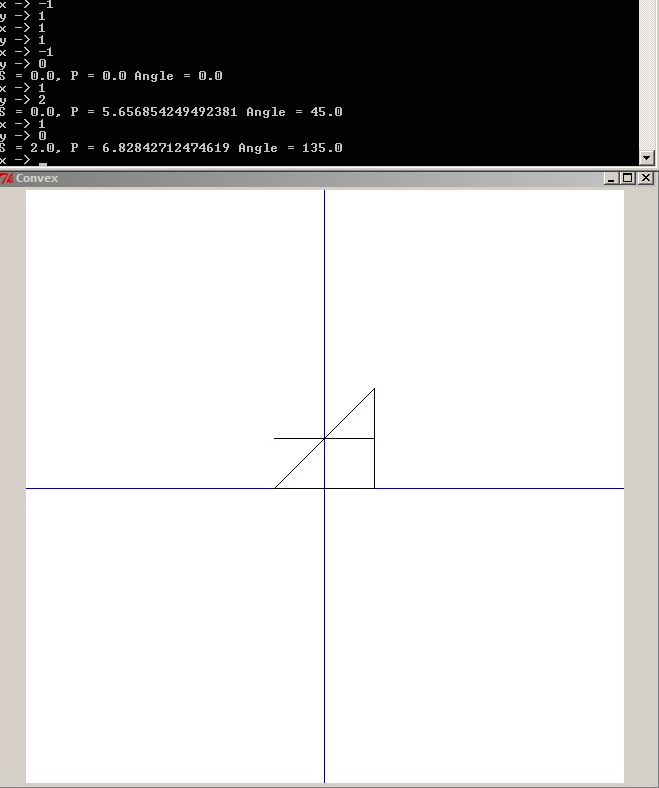
\includegraphics[width=0.8\hsize]{images/screen1}
\end{center}
\caption{Работа программы «Выпуклая оболочка»}
\end{figure}












